\documentclass[journal]{IEEEtran}

\usepackage{amsmath,amssymb,amsfonts}
\usepackage{graphicx}
\usepackage{booktabs}
\usepackage{multirow}
\usepackage{url}
\usepackage{cite}
\usepackage{subcaption}
\usepackage{xcolor}
\usepackage{hyperref}
\hypersetup{colorlinks=true, citecolor=green, linkcolor=red, urlcolor=blue}

\begin{document}

\title{Quantifying Anthropometric Leakage in Obesity Risk Classification and It's Implications for Threshold-Defined Labels in Clinical Machine Learning}

\author{\textit{
\IEEEauthorblockN{Frank Anokye{$^{1}$}\\
\IEEEauthorblockA{University of L'Aquila, Italy, L,Aquila \\ Silesian University of Technology, Poland, Gliwice }}}}


%\markboth{Preprint, submitted for review}{}

\maketitle

\begin{abstract}
Studies using the Fabio Mendoza Palechor and Alexis de la Hoz Manotas obesity dataset (2{,}111 records, 17 attributes) generally report classification accuracy above 90\% to 96\%. This is often presented as evidence that machine learning can predict the risk of obesity from behavior. We show that this apparent performance comes mainly from something simpler. The seven level obesity target in this dataset is assigned using fixed body mass index (BMI) thresholds, and BMI is an exact algebraic function of two features already in the predictor set, Weight and Height. A classifier that has access to these two features can solve largely an arithmetic threshold recovery problem rather than a genuine behavior prediction problem. We clearly state this distinction and test two separate tasks on the same data, one using the full feature set and another using only lifestyle, dietary, and demographic features, with Weight, Height, and BMI removed. Using six classifier types, each carefully tuned and cross validated, with a stacking ensemble, we get 97.8\% test accuracy (macro F1 of 0.978) on the full feature task and 86.1\% test accuracy (macro F1 of 0.857) on the lifestyle only task. We also show, using SHAP, that vegetable consumption frequency, age, gender, and family history of overweight individuals are the strongest lifestyle predictors of the obesity risk category. A parallel regression analysis that predicts continuous BMI from lifestyle features alone reaches an $R^{2}$ of 0.869 using a tuned random forest, compared to about 0.46 for regularized linear models, a large improvement over a prior linear regression baseline that reached only 0.207. A cluster validity analysis (silhouette score, Davies Bouldin index, adjusted Rand index) shows that the natural structure of the feature space lines up only weakly with the seven class labeling scheme, with an adjusted Rand index of 0.179. This tells us that the class boundaries are cutoffs chosen by researchers rather than groups that emerge naturally from the data. We argue that this distinction between diagnostic and behavioral tasks should be standard practice whenever this dataset, or similarly built obesity datasets, is used for obesity risk research.
%and we release a fully reproducible, path independent codebase to support that.
\end{abstract}

\begin{IEEEkeywords}
Obesity classification, machine learning, data leakage, explainable AI, SHAP, stacking ensemble, class imbalance, body mass index, health informatics.
\end{IEEEkeywords}

\section{Introduction}
\label{sec:intro}

Obesity is a major public health problem worldwide. In 2022, an estimated 2.5 billion adults were overweight and 890 million of them were living with obesity. Global obesity rates have more than doubled since 1990 \cite{who2024obesity, ncdrisc2024}. Because obesity depends on many things at once, including diet, physical activity, family history, and social and economic context, there has been strong and lasting interest in using machine learning to find out which behavioral and lifestyle factors matter most, with the goal of building economically scalable tools for screening and early intervention \cite{freitas2024metaanalysis}.

Much of this research reuses a single public dataset, the  Fabio Mendoza Palechor and Alexis de la Hoz Manotas obesity dataset, titled Estimation of obesity levels based on eating habits and physical condition, collected from 498 people in Colombia, Peru, and Mexico through a web survey and expanded to 2{,}111 records using the SMOTE based synthetic oversampling technique \cite{palechor2019dataset, chawla2002smote}. The classification accuracy reported on this dataset is consistently high. The corresponding decision tree study reports strong results \cite{delahoz2019obesity}. A 2025 benchmarking study using SHAP based interpretability reports 95.9\% accuracy with gradient boosting and 97.9\% with a stacking ensemble \cite{benchmarking2025shap}. Other studies report similarly high numbers using logistic regression, random forests, and XGBoost \cite{ratih2019estimation}.

We think these high accuracy numbers, while technically correct, overstate how hard the underlying prediction problem actually is, and overstate how useful these models are for behavioral screening, for a reason that has not been clearly stated in this literature, the target label in this dataset is built from BMI using fixed thresholds, and the predictor set includes Weight and Height, from which BMI is an exact formula ($\frac{\mathrm{Weight}}{\mathrm{Height}^2}\,$). A small number of earlier studies have implicitly noticed a related concern by leaving out BMI adjacent features to focus on lifestyle variables \cite{oyelude2023lifestyle}, but this choice, and what it actually does to reported performance, is rarely stated directly or measured within a single study.

\subsection{What This Paper Contributes}
This paper started as a re-analysis and extension of earlier exploratory coursework that applied a single, untuned decision tree, a plain linear regression, and a KMeans clustering with a fixed number of clusters to this dataset. Building on that starting point, this paper:

\begin{itemize}
\item State clearly how the anthropometric leakage in the Palechor and de la Hoz Manotas dataset works (Section~\ref{sec:leakage}), and measure its effect on classification accuracy by testing matched model types under two conditions, notably, a diagnostic condition using the full feature set, and a behavioral risk condition with Weight, Height, and BMI removed.
\item Use a careful, leak free model selection and testing process, which are, stratified train and test splitting, five fold cross validated randomized hyperparameter search for six base learner types, and a stacking ensemble \cite{wolpert1992stacked} that combines the strongest base learners through a logistic regression meta learner, tested once on a held out test set.
\item Measure the effect of correcting for class imbalance (class weighting and SMOTE oversampling, both applied only inside cross validation folds) and show that this dataset's imbalance is mild, so correction gives only modest gains, contrary to an assumption made without testing in some earlier work.
\item Apply SHAP \cite{lundberg2017shap} to the behavioral risk model specifically, rather than the diagnostic model, whose feature importances would just show Weight and Height as dominant and add no real insight, to find out which modifiable lifestyle factors matter most.
\item Reformulate the continuous outcome regression task as predicting BMI from lifestyle features alone, with proper cross validation and a comparison of regularized linear models against ensemble models, substantially improving on the original coursework's regression fit.
\item Check the natural cluster structure of the feature space against the labels used in the dataset, using silhouette scores \cite{rousseeuw1987silhouettes}, the Davies Bouldin index \cite{daviesbouldin1979}, and the adjusted Rand index, rather than fixing the number of clusters in advance.
\item Produce a fully reproducible codebase (Section~\ref{sec:repro}) in which every script finds its own files based on where it is saved on disk, so the whole pipeline can be run again, exactly, by anyone, on any computer, with no changes to any file path.
\end{itemize}

\section{Related Work}
\label{sec:related}

\cite{palechor2019dataset} released the dataset along with an associated decision tree-based estimation tool \cite{delahoz2019obesity}. The dataset combines 23\% directly surveyed responses with 77\% synthetic records generated using SMOTE \cite{chawla2002smote} in Weka, specifically to balance an originally skewed class distribution.

Many studies benchmark classical and ensemble classifiers on this dataset. \cite{ratih2019estimation} compare logistic regression, random forest, and XGBoost. A recent benchmarking study \cite{benchmarking2025shap} compares six classifiers with SMOTE based balancing and SHAP interpretability, reporting a best gradient boosting accuracy of 95.9\% and a stacking ensemble accuracy of 97.9\%, strikingly close to our own full feature stacking result of 97.8\% (Section~\ref{sec:results-taskA}). We take that closeness as independent support for the idea that a diagnostic task accuracy ceiling near 97\% to 98\% percent is a stable, repeatable property of this dataset's full feature set. \cite{oyelude2023lifestyle} explicitly restrict their feature set to lifestyle variables to avoid relying on BMI, a choice that lines up with the behavioral task we define below. What this paper adds beyond their work is a direct, controlled comparison between the full feature and lifestyle only settings within a single study, which their paper does not report.

A 2024 systematic review and meta analysis of machine learning obesity prediction across cohort studies found random forest to be the strongest average performer, with a pooled area under the curve of 0.86, just ahead of logistic regression at 0.85, while gradient boosting performed comparatively worse, at 0.77, in that pooled sample \cite{freitas2024metaanalysis}. We do not fully see the same pattern on this dataset, where boosting and its stacking ensemble combination are highly competitive. This suggests that which method works best for obesity prediction depends on the specific dataset and its leakage structure, rather than reflecting one universal ranking of model quality. Our approach uses random forests \cite{breiman2001randomforests}, gradient boosting \cite{friedman2001gradientboosting}, support vector machines \cite{cortes1995svm}, stacked generalization \cite{wolpert1992stacked}, SHAP \cite{lundberg2017shap}, SMOTE \cite{chawla2002smote}, and standard cluster validity measures \cite{rousseeuw1987silhouettes, daviesbouldin1979}, implemented using scikit-learn \cite{scikit-learn}.

\section{Problem Definition}
\label{sec:leakage}

\subsection{Setting Up the Problem}
Let $\mathbf{x} = (x_1, \ldots, x_{16}) \in \mathcal{X}$ be the predictor values for one person, made up of eight numeric features (Age, Height, Weight, FCVC, NCP, CH2O, FAF, TUE) and eight categorical features (Gender, family history of overweight, FAVC, CAEC, SMOKE, SCC, CALC, MTRANS), and let $y \in \mathcal{Y}$ be the ordinal obesity class, $\mathcal{Y} = \{$Insufficient\_Weight, Normal\_Weight, Overweight\_Level\_I, Overweight\_Level\_II, Obesity\_Type\_I, Obesity\_Type\_II, Obesity\_Type\_III$\}$.

\subsection{How the Anthropometric Leakage Works}
Define BMI as
\begin{equation}
\mathrm{BMI}(\mathbf{x}) = \frac{\mathrm{Weight}}{\mathrm{Height}^2}\,, \qquad [\mathrm{kg/m^2}].
\label{eq:bmi}
\end{equation}
Looking at the cleaned dataset (Section~\ref{sec:data}), the BMI range for each class works out as follows.
\begin{align}
&\text{Insufficient\_Weight: } [13.0,19.1),\quad \text{Normal\_Weight: } [18.5,24.9), \nonumber\\
&\text{Overweight\_I: } [22.8,28.8),\quad \text{Overweight\_II: } [25.7,30.4), \nonumber\\
&\text{Obesity\_I: } [29.9,35.2),\quad \text{Obesity\_II: } [34.0,39.8), \nonumber\\
&\text{Obesity\_III: } [36.8,50.8). \nonumber
\end{align}
These ranges barely overlap, and they line up closely with standard WHO and regional BMI category cutoffs. This confirms that $y$ is, to a close approximation, a fixed step function of BMI:
\begin{equation}
y \approx g\!\big(\mathrm{BMI}(\mathbf{x})\big), \qquad g:\mathbb{R}_{+}\to\mathcal{Y}\ \text{piecewise constant.}
\label{eq:leakage}
\end{equation}
Because Weight and Height are themselves part of $\mathbf{x}$, any classifier $f: \mathcal{X}\to\mathcal{Y}$ with access to the full feature vector can, in principle, approximate $g$ applied to BMI directly, without using any information about diet, activity, or family history. We call this the anthropometric leakage structure of the dataset. This is not a flaw in the data. Labeling by BMI is a normal and defensible clinical practice. But it means that classification accuracy under the full feature set measures how well a model recovers a known arithmetic threshold rule, not how well behavioral and demographic factors predict obesity risk on their own.

\subsection{Two Research Questions}
We therefore look at two tasks that share the same underlying population.

\textbf{Task A, diagnostic classification.} Given the full feature vector $\mathbf{x}$, including Weight and Height, predict $y$. This is the setup used, either stated or not, in most earlier work on this dataset (Section~\ref{sec:related}).

\textbf{Task B, behavioral risk classification.} Given $\mathbf{x}^{-} = \mathbf{x}\setminus\{\mathrm{Weight}, \mathrm{Height}, \mathrm{BMI}\}$, predict $y$. This isolates the genuinely open question, how much of obesity category membership can be predicted from modifiable lifestyle and demographic factors alone, without a direct anthropometric measurement.

We test both tasks under the same rigorous model selection process (Section~\ref{sec:methods}), which lets us directly measure the leakage effect, $\Delta = \mathrm{Perf}(\text{Task A}) - \mathrm{Perf}(\text{Task B})$. As far as we know, this has not been reported for this dataset in earlier published work.

\section{Data}
\label{sec:data}

\subsection{Source and What It Contains}
We use the public Palechor and de la Hoz Manotas dataset \cite{palechor2019dataset}, with 2{,}111 records and 17 attributes, 16 predictors and the target NObeyesdad, of which 77\% were generated using SMOTE oversampling and 23\% were directly surveyed \cite{palechor2019dataset, chawla2002smote}. We suggest that this should be stated clearly whenever this dataset is used, since downstream models are partly learning from synthetic, interpolated data rather than only from directly observed records. We treat this as a limitation (Section~\ref{sec:limitations}) rather than leaving it out.

\subsection{Cleaning}
We found 24 exact duplicate rows using a full row comparison, which we removed, leaving 2{,}087 records. We note that an earlier analysis of this same file reported zero duplicates, which we could not reproduce using a standard check. We think this is because SMOTE based synthetic generation can occasionally produce identical rows. No values were missing. Feature ranges (Age 14 to 61 years, Height 1.45 to 1.98 meters, Weight 39 to 173 kilograms) were checked and found to be reasonable.

\subsection{New Features}
We compute BMI using Equation~\eqref{eq:bmi} for description and as the regression target in Section~\ref{sec:regression}. Ordinal categorical variables (CAEC, CALC, with levels Never, Sometimes, Frequently, Always) are coded in order rather than dummy encoded, keeping their natural order; the nominal variable MTRANS is dummy encoded; binary variables are coded as single indicator columns.

\section{Methods}
\label{sec:methods}

\subsection{Statistical Testing}
For each numeric feature $x_j$, we test whether the class averages are equal using a one way ANOVA,
\begin{equation}
F = \frac{\mathrm{MS}_{\text{between}}}{\mathrm{MS}_{\text{within}}} = \frac{\sum_{k=1}^{7} n_k (\bar{x}_k - \bar{x})^2 / (7-1)}{\sum_{k=1}^{7}\sum_{i \in k} (x_{ij}^{(i)} - \bar{x}_k)^2 / (n-7)},
\label{eq:anova}
\end{equation}
along with a non-parametric Kruskal Wallis test as a check on the normality and equal variance assumptions behind Equation~\eqref{eq:anova}, and an effect size, $\eta^2 = \mathrm{SS}_{\text{between}}/\mathrm{SS}_{\text{total}}$. For categorical features, we use Pearson's $\chi^2$ test of independence with Cramer's V effect size. Because 17 hypothesis tests are run, we control the false discovery rate at $q=0.05$ using the Benjamini Hochberg procedure \cite{benjaminihochberg1995}, sorting p-values $p_{(1)} \le \cdots \le p_{(m)}$ and rejecting $H_{0,(i)}$ for all $i \le \max\{i : p_{(i)} \le \frac{i}{m}q\}$.

\subsection{Preprocessing}
All preprocessing (median imputation, z-score standardization of numeric features, dummy or ordinal encoding of categorical features) is done using an \texttt{sklearn.compose.ColumnTransformer} fit only on training folds within cross validation, so no test fold information leaks into scaling or encoding.

\subsection{Classification Models and Tuning}
\label{sec:clf-methods}
We test six base learner types, L2 regularized multinomial logistic regression, k-nearest neighbors, RBF kernel support vector machines \cite{cortes1995svm}, decision trees, random forests \cite{breiman2001randomforests}, and histogram based gradient boosting \cite{friedman2001gradientboosting}. For each, hyperparameters are tuned using a randomized search, 25 candidate settings multiplied  by five fold stratified cross validation, scored on macro averaged F1, on an 80\% training split, with the remaining 20\% held out, stratified by class, and used only once, at the end, for final testing. We use macro F1 as the tuning target because all seven classes matter equally for this problem, regardless of their mildly unequal sample sizes.

A stacking ensemble \cite{wolpert1992stacked} is then built from the three strongest base learners by cross validated score, combined through a logistic regression meta learner trained on out of fold base learner predictions, five fold, which is the standard leak free stacking procedure. This full process, tuning, stacking, and testing, is applied the same way to Task A and Task B.

\subsection{Testing Class Imbalance Correction}
The target distribution ranges from 272 records, Insufficient\_Weight, to 351 records, Obesity\_Type\_I, a ratio of 1.29 to 1, which is mild imbalance. We still test three strategies under identical five fold cross validation on Task B: no correction, inverse frequency class weighting, and SMOTE oversampling \cite{chawla2002smote}, applied only inside each training fold using an imbalanced-learn pipeline, never before the train and test split, which would otherwise leak synthetic near duplicate information across the split.

\subsection{Explainability}
We compute SHAP values \cite{lundberg2017shap} using TreeExplainer on the best tree based Task B model, averaging the absolute SHAP value across the seven output classes over a 300 sample test subset, to get an overall feature importance ranking. We explain the Task B, or behavioral, model specifically. Explaining the Task A model would, given the leakage structure in Section~\ref{sec:leakage}, just rank Weight and Height as dominant and add no real insight.

\subsection{Regression}
\label{sec:regression}
We predict continuous BMI (Equation~\eqref{eq:bmi}) from the same lifestyle only predictor set used in Task B, with Weight and Height also excluded, since they are BMI's algebraic components. We compare ordinary least squares, ridge regression, and lasso regression, with regularization strength tuned by randomized search, against a tuned random forest regressor, under five fold cross validation with a held out 20\% test set, reporting $R^{2}$, MAE, and RMSE.

\subsection{Cluster Validity}
We run KMeans over $k \in \{2,\ldots,10\}$ on the fully processed feature matrix (Task A features), choosing $k$ by maximizing the silhouette score \cite{rousseeuw1987silhouettes}, checked against the Davies Bouldin index \cite{daviesbouldin1979} and the inertia elbow, rather than fixing $k$ in advance. We also compute the adjusted Rand index (ARI) and normalized mutual information (NMI) between the clusters and the true seven class label, to measure how much of the natural unsupervised structure matches the imposed clinical classes.

\section{Experiments and Results}
\label{sec:results}

\subsection{Basic Statistics and Hypothesis Tests}
Table~\ref{tab:desc} summarizes the numeric predictors. All eight numeric features and all eight categorical features are significantly associated with obesity class after Benjamini Hochberg correction ($p_{\mathrm{BH}} < 0.05$ throughout; for example, Weight: $F=1926.5$, $p \approx 0$; FCVC: $F=110.5$, $p_{\mathrm{BH}} \approx 1.1\times10^{-120}$; Gender: $\chi^2=657.5$, $p_{\mathrm{BH}} \approx 4.0\times10^{-138}$), confirming that the dataset carries real, statistically solid signal beyond the anthropometric variables alone.

\begin{table}[t]
\centering
\caption{Basic statistics for the numeric predictors and BMI ($n=2{,}087$, after cleaning).}
\label{tab:desc}
\begin{tabular}{lrrrr}
\toprule
Feature & Mean & SD & Min & Max \\
\midrule
Age (yr) & 24.35 & 6.37 & 14.0 & 61.0 \\
Height (m) & 1.70 & 0.09 & 1.45 & 1.98 \\
Weight (kg) & 86.86 & 26.19 & 39.0 & 173.0 \\
FCVC & 2.42 & 0.53 & 1.0 & 3.0 \\
NCP & 2.70 & 0.76 & 1.0 & 4.0 \\
CH2O & 2.00 & 0.61 & 1.0 & 3.0 \\
FAF & 1.01 & 0.85 & 0.0 & 3.0 \\
TUE & 0.66 & 0.61 & 0.0 & 2.0 \\
BMI (kg/m$^2$) & 29.77 & 8.02 & 12.99 & 50.81 \\
\bottomrule
\end{tabular}
\end{table}

\subsection{Task A: Diagnostic Classification (Full Feature Set)}
\label{sec:results-taskA}
Table~\ref{tab:clfA} reports held out test performance. Gradient boosting, at 95.7\% percent cross validated macro F1, and random forest, at 93.8\%, were the strongest individual base learners. The stacking ensemble, which combines gradient boosting, random forest, and logistic regression base learners, gave the best held out performance: 97.8\% accuracy, macro F1 of 0.978. This matches the high accuracy numbers reported in earlier work using the full feature set \cite{benchmarking2025shap, ratih2019estimation, delahoz2019obesity}, and fits with the leakage explanation in Section~\ref{sec:leakage} recovering a BMI threshold rule from Weight and Height, given consistent synthetic data, is a comparatively easy learning problem.

\begin{table}[t]
\centering
\caption{Task A (full feature set) held out test performance.}
\label{tab:clfA}
\begin{tabular}{lrrr}
\toprule
Model & Accuracy & Macro F1 & Bal. Acc. \\
\midrule
\textbf{Stacking Ensemble} & \textbf{0.978} & \textbf{0.978} & \textbf{0.978} \\
Gradient Boosting & 0.974 & 0.973 & 0.973 \\
Decision Tree & 0.962 & 0.961 & 0.962 \\
Random Forest & 0.955 & 0.954 & 0.953 \\
SVM (RBF) & 0.940 & 0.937 & 0.937 \\
Logistic Regression & 0.938 & 0.935 & 0.937 \\
$k$-NN & 0.854 & 0.841 & 0.847 \\
\bottomrule
\end{tabular}
\end{table}

\subsection{Task B: Behavioral Risk Classification (Lifestyle Only)}
\label{sec:results-taskB}
Table~\ref{tab:clfB} reports the same process with Weight, Height, and BMI removed. Performance drops in an informative way: the best model, random forest, reaches 86.1\% accuracy and a macro F1 of 0.857, a leakage effect of $\Delta_{\text{accuracy}} = 0.978 - 0.861 = 0.117$ (11.7 percentage points) and $\Delta_{\text{macro-}F_1} = 0.121$. The stacking ensemble did not beat its best base learner, random forest, on Task B, unlike on Task A. This suggests that once the anthropometric signal is removed, one strong tree ensemble already captures most of the remaining predictive information, and stacking gives little extra benefit. Logistic regression drops sharply (macro F1 of 0.554), which tells us the relationship between lifestyle and outcome is far from a straight line.

\begin{table}[t]
\centering
\caption{Task B (lifestyle only feature set) held out test performance.}
\label{tab:clfB}
\begin{tabular}{lrrr}
\toprule
Model & Accuracy & Macro F1 & Bal. Acc. \\
\midrule
\textbf{Random Forest} & \textbf{0.861} & \textbf{0.857} & \textbf{0.856} \\
Stacking Ensemble & 0.859 & 0.856 & 0.854 \\
Gradient Boosting & 0.847 & 0.842 & 0.843 \\
SVM (RBF) & 0.792 & 0.793 & 0.787 \\
$k$-NN & 0.768 & 0.747 & 0.760 \\
Decision Tree & 0.737 & 0.730 & 0.734 \\
Logistic Regression & 0.591 & 0.554 & 0.577 \\
\bottomrule
\end{tabular}
\end{table}

\subsection{Class Imbalance Correction}
Table~\ref{tab:imbalance} confirms what we would expect given the mild, 1.29 to 1, imbalance ratio. Class weighting and SMOTE oversampling give small, consistent improvements, macro F1 going from 0.842 to 0.847 to 0.849, rather than large gains. Per class recall, given in full in the supplementary file \texttt{results/imbalance\_strategy\_comparison.csv}, shows the class most sensitive to correction is Normal\_Weight, with recall going from 0.724 to 0.751 under SMOTE, the class most easily confused with its neighboring categories.

\begin{table}[t]
\centering
\caption{Class imbalance correction strategies, five fold cross validation on Task B training split.}
\label{tab:imbalance}
\begin{tabular}{lrr}
\toprule
Strategy & Macro F1 & Balanced Accuracy \\
\midrule
None (baseline) & 0.842 & 0.842 \\
Class weighting & 0.847 & 0.847 \\
SMOTE oversampling & 0.849 & 0.849 \\
\bottomrule
\end{tabular}
\end{table}

\subsection{Explainability: What Drives Behavioral Risk Predictions}
Figure~\ref{fig:shap} shows overall SHAP feature importance for the Task B random forest. The strongest modifiable predictors are frequency of vegetable consumption (FCVC), age, gender, and family history of overweight, followed by number of main meals (NCP), eating between meals (CAEC), technology use time (TUE), and alcohol consumption frequency (CALC). Physical activity frequency (FAF) ranks lower than commonly assumed, suggesting that in this population, dietary pattern and family history carry more useful signal than exercise frequency once anthropometric variables are removed, though we are careful not to treat this as a causal claim (Section~\ref{sec:discussion}).

\begin{figure}[t]
\centering
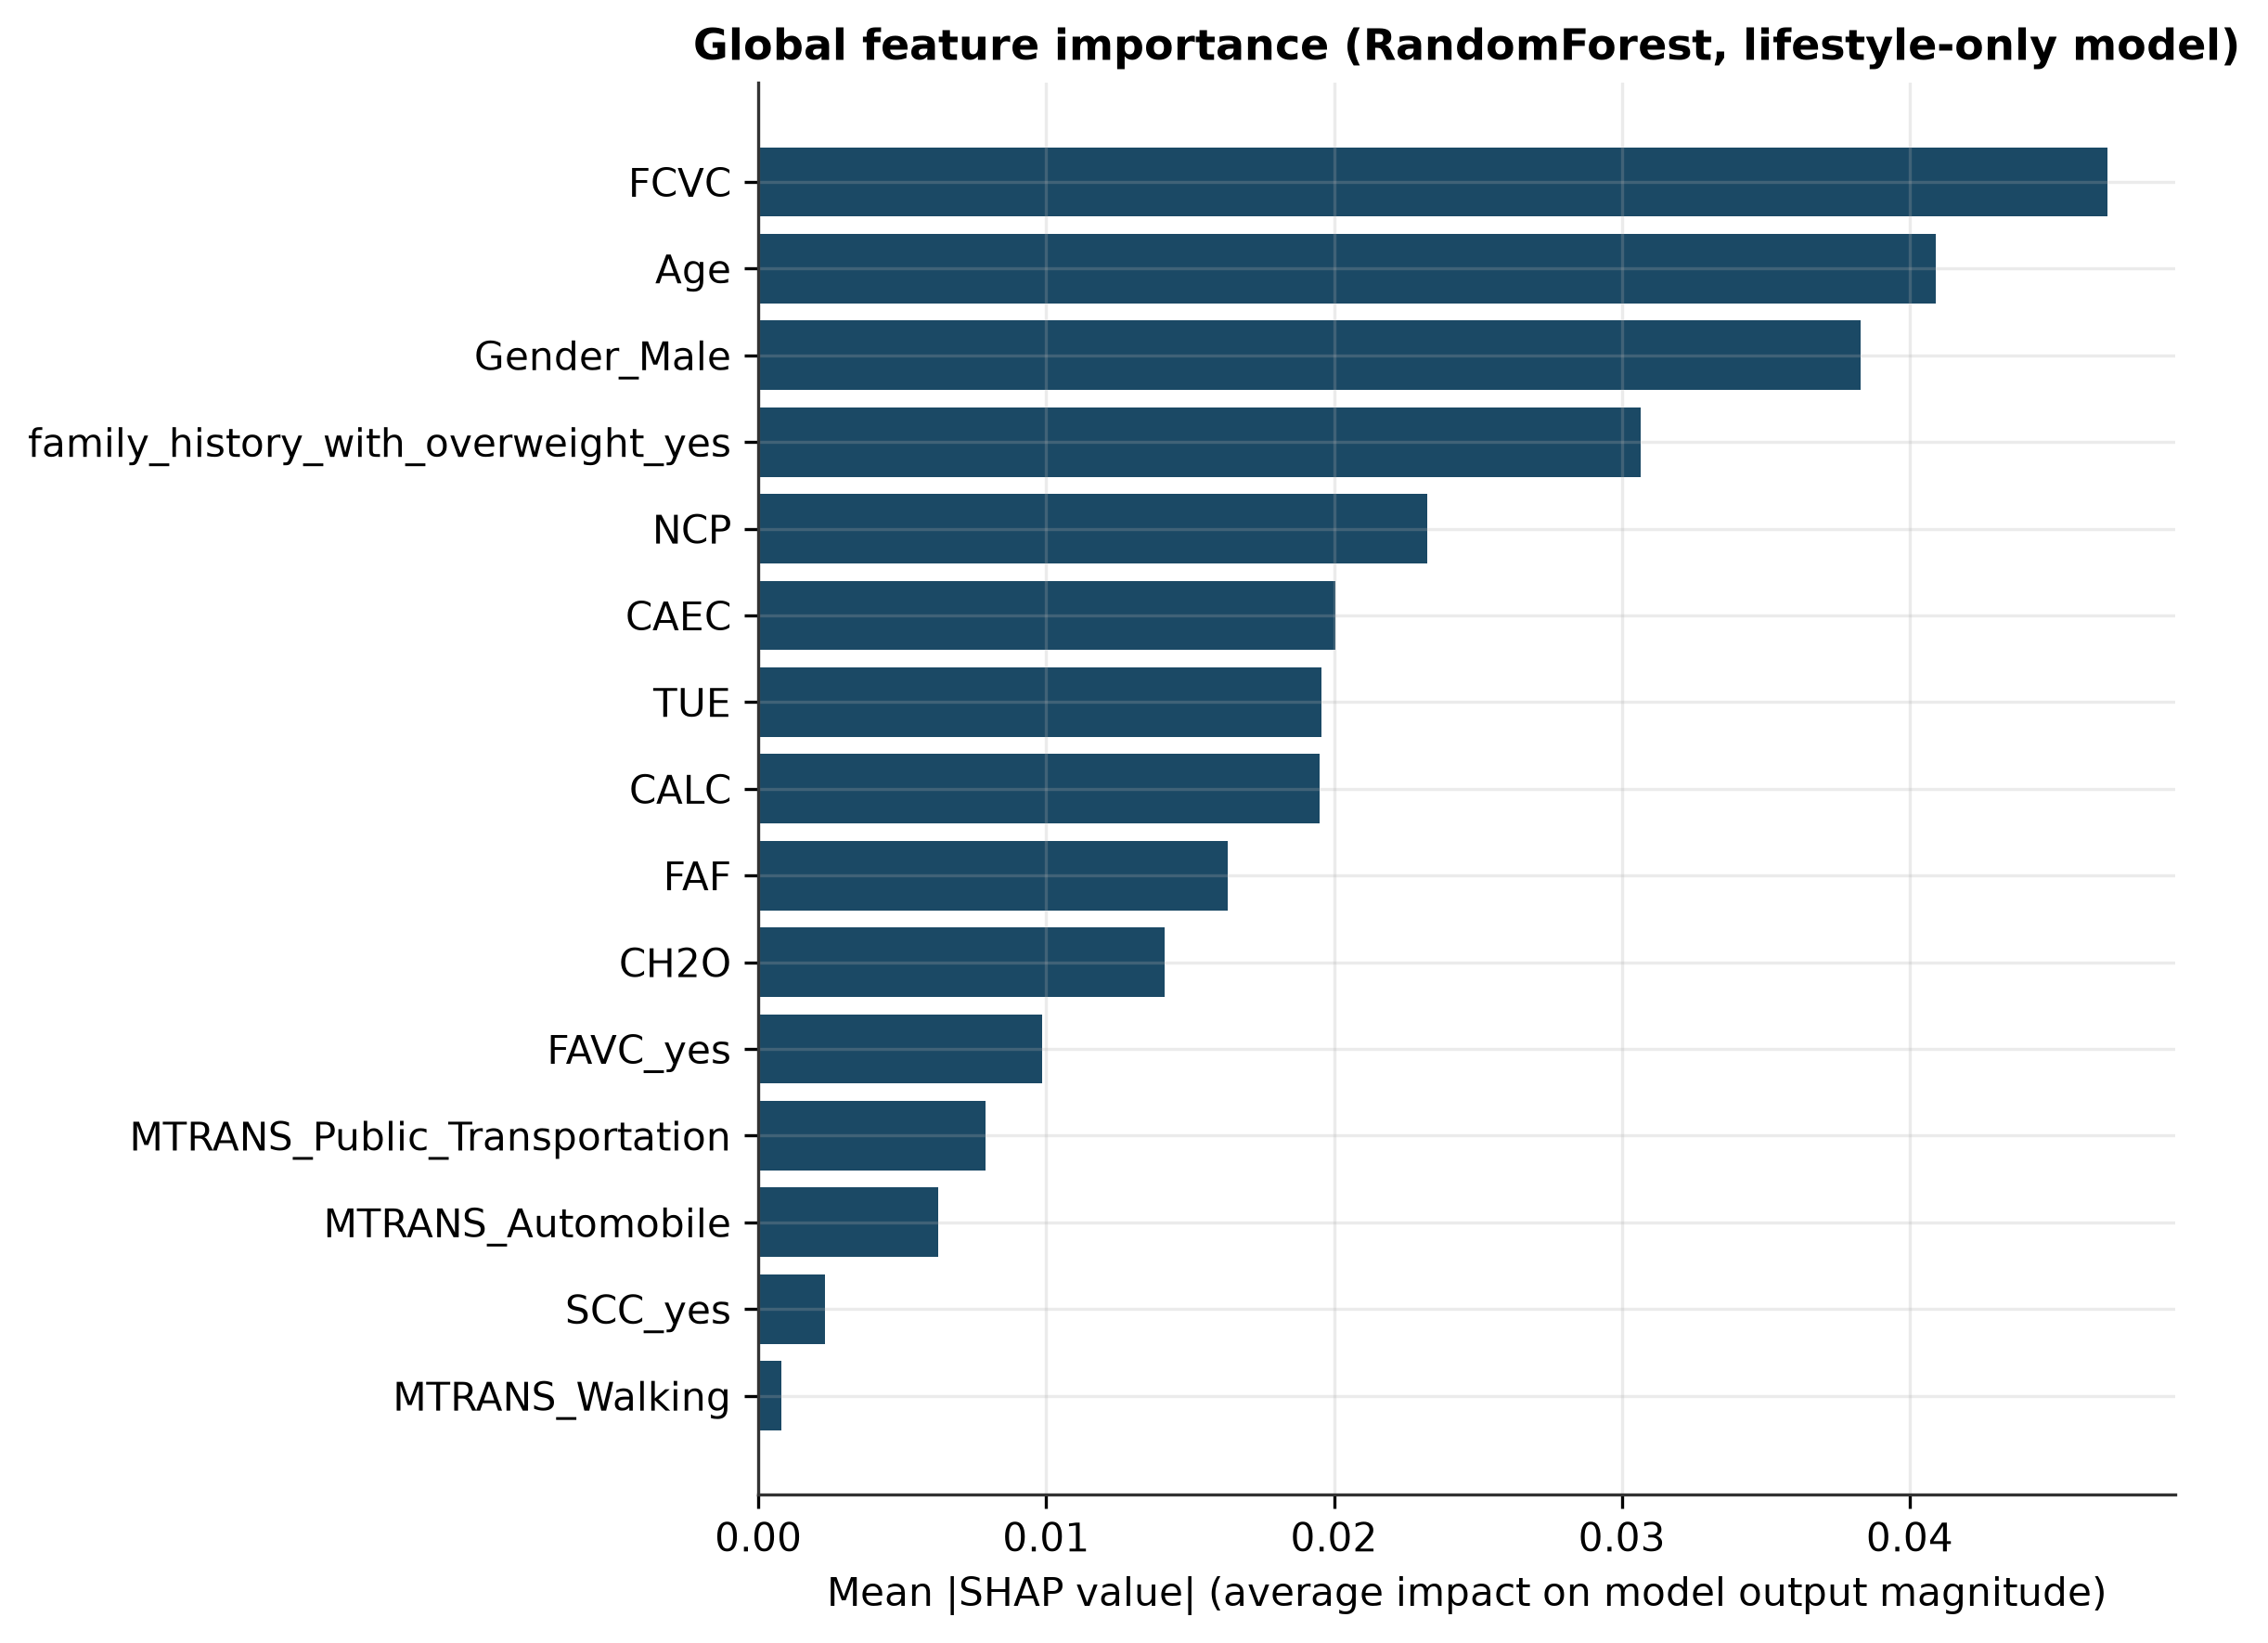
\includegraphics[width=\columnwidth]{../figures/fig12_shap_feature_importance.png}
\caption{Overall SHAP feature importance, Task B (lifestyle only) random forest classifier.}
\label{fig:shap}
\end{figure}

\subsection{Regression: Predicting Continuous BMI from Lifestyle Factors}
Table~\ref{tab:reg} reports BMI regression results. The tuned random forest regressor reaches a test $R^{2} $of 0.869 (RMSE 2.93 kg/m$^2$, MAE 1.88 kg/m$^2$), a large improvement over regularized linear models, around 0.46, and over the original coursework's linear regression baseline on the ordinal class target, 0.207. Figure~\ref{fig:reg} shows predicted versus true BMI and residuals for the best model. Residuals show mild spread at high BMI, which fits with greater behavioral variety among people with more severe obesity.

\begin{table}[t]
\centering
\caption{BMI regression, lifestyle only predictors, held out test set.}
\label{tab:reg}
\begin{tabular}{lrrr}
\toprule
Model & $R^2$ & MAE (kg/m$^2$) & RMSE (kg/m$^2$) \\
\midrule
\textbf{Random Forest} & \textbf{0.869} & \textbf{1.88} & \textbf{2.93} \\
Lasso & 0.462 & 4.75 & 5.94 \\
Ridge & 0.462 & 4.72 & 5.94 \\
OLS & 0.460 & 4.73 & 5.95 \\
\bottomrule
\end{tabular}
\end{table}

\begin{figure}[t]
\centering
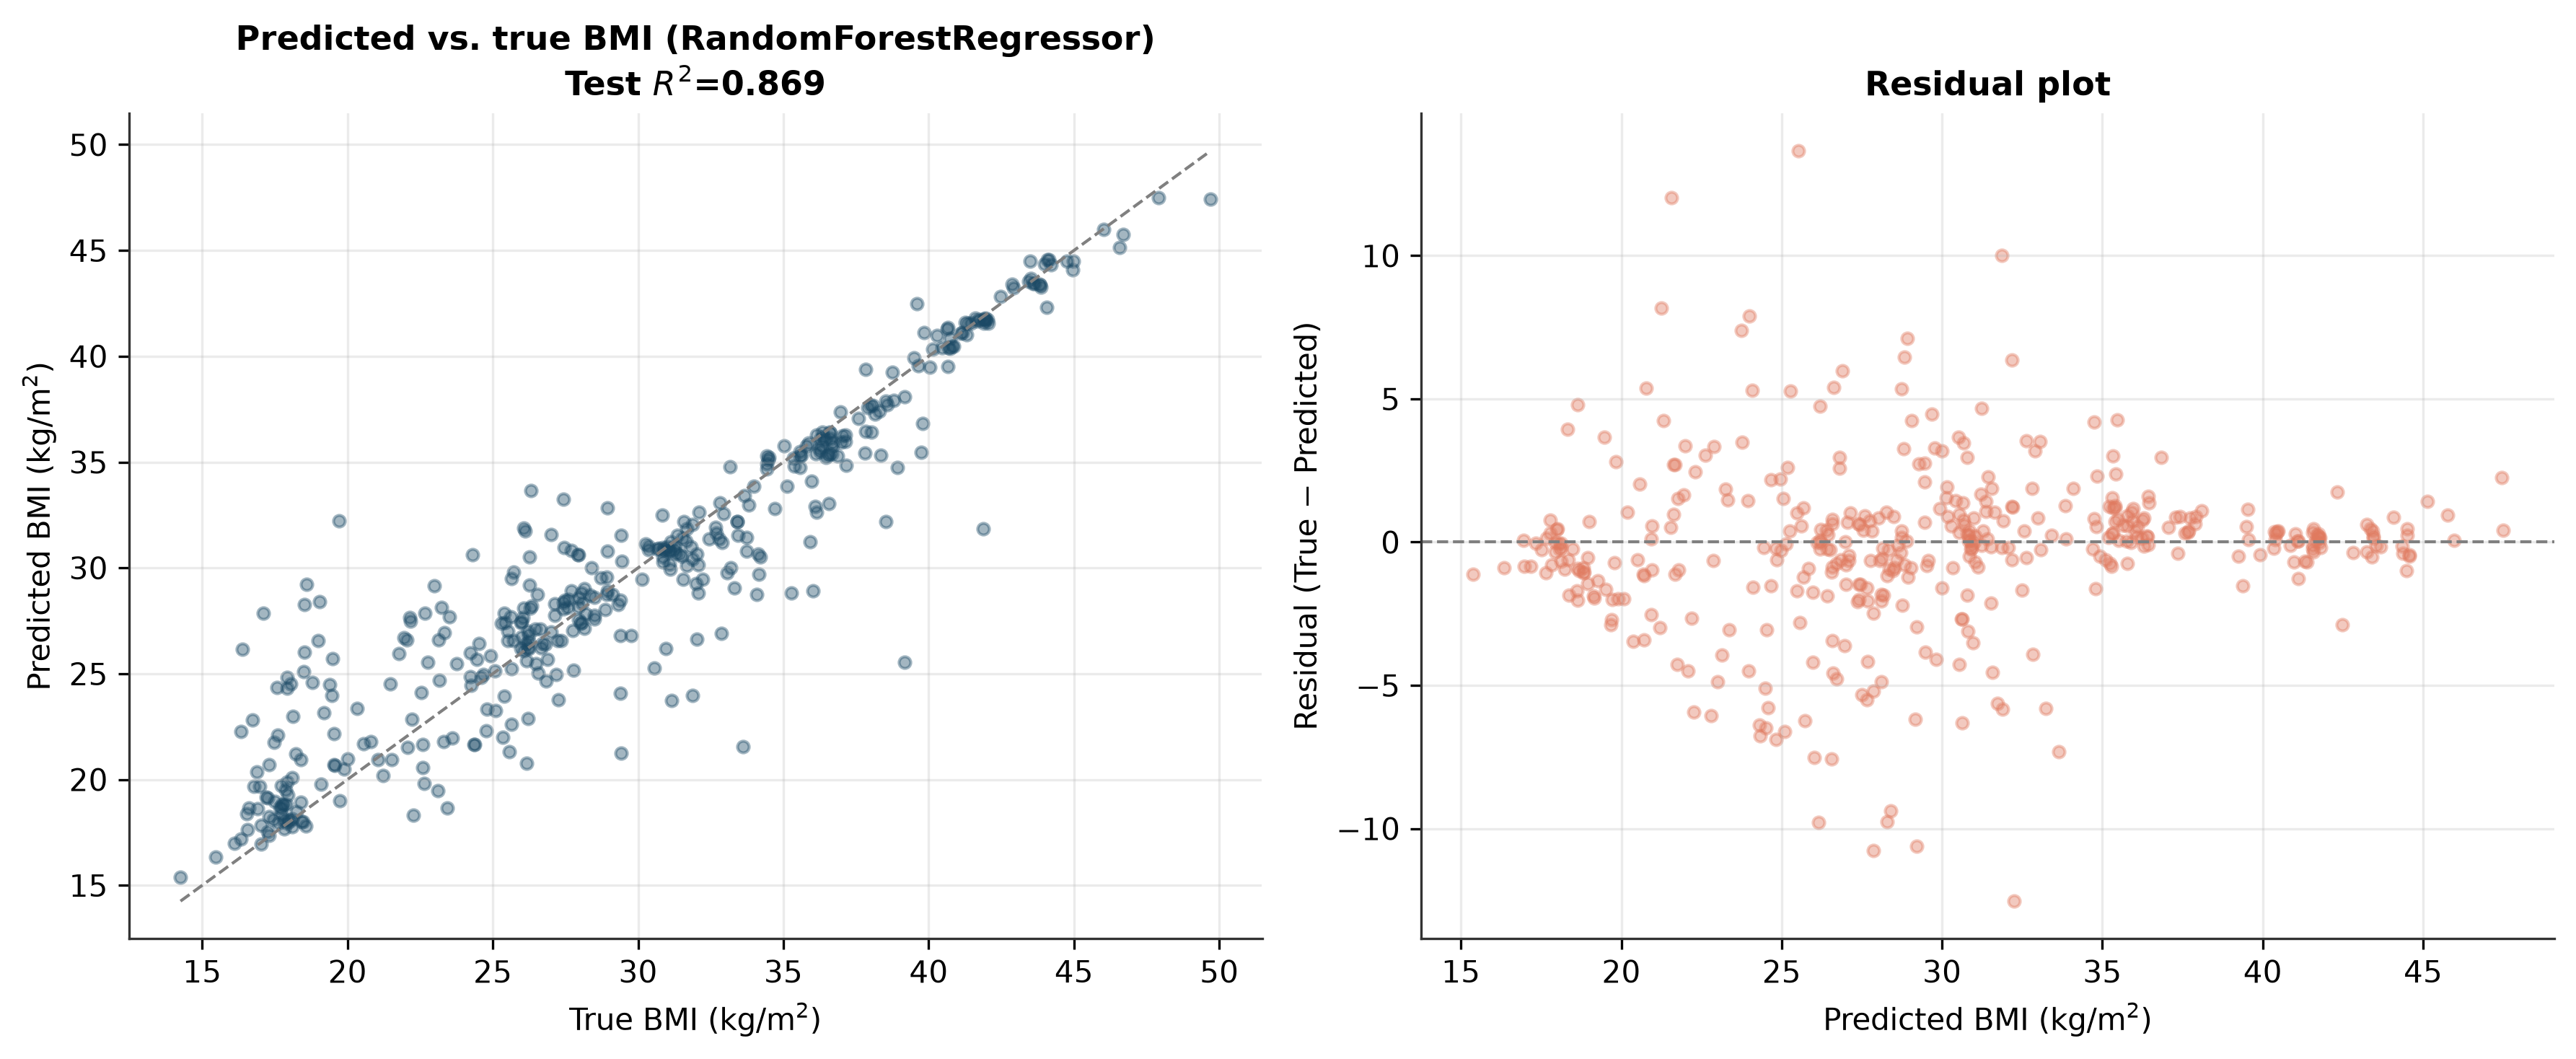
\includegraphics[width=\columnwidth]{../figures/fig13_regression_bmi_prediction.png}
\caption{Predicted versus true BMI, and residuals, tuned random forest regressor, lifestyle only predictors.}
\label{fig:reg}
\end{figure}

\subsection{Cluster Validity}
Checking $k\in\{2,\ldots,10\}$, the silhouette score picks $k=4$ as best (silhouette $=0.155$, Davies Bouldin $=1.977$), unlike the original coursework's fixed choice of $k=5$, which was never explained. The low silhouette value tells us the feature space does not split into naturally separated groups, which fits with obesity being more of a continuum than a set of distinct clusters. Agreement with the true seven class label is weak (ARI $=0.179$, NMI $=0.247$), confirming that the class boundaries are cutoffs chosen by researchers rather than structure that emerges naturally from the joint feature distribution.

\section{Discussion}
\label{sec:discussion}
The main finding of this study is that about 11\% to 12\% points of the headline accuracy usually reported for this dataset come from anthropometric leakage rather than genuine behavioral predictability. This matters for two practical reasons. First, for diagnostic use, such as automating BMI category assignment from an intake form that already records height and weight, Task A models are appropriate and work well. Second, for screening or risk communication use, where the goal is to predict obesity risk from modifiable behavior before, or instead of, a direct measurement, such as a lifestyle questionnaire used in a population level screening program, Task B is the scientifically honest formulation. Its accuracy of 86\%, macro F1 0.857, while still strong, should be the reported and interpreted benchmark, not the 97.8\% figure. We recommend that future studies using this dataset state clearly which task they are actually solving.

The SHAP results (Figure~\ref{fig:shap}) should be read as showing predictive importance within this cross sectional, partly synthetic sample, not as causal effect estimates. In particular, the modest ranking of physical activity (FAF) relative to dietary variables (FCVC, NCP, CAEC) may partly reflect self report measurement noise, the specific survey population (Colombia, Peru, Mexico), or non-linear interaction effects not fully captured by averaging absolute SHAP values across classes.

\section{Limitations}
\label{sec:limitations}
First, synthetic data. 77\% of records are SMOTE generated \cite{palechor2019dataset}, so models are partly learning from interpolated rather than directly observed people, which may make predictability higher than it would be in a purely observational sample of the same size. Second, self report bias. All behavioral variables (FCVC, FAF, CAEC, etc.) are self reported through a web survey, with no independent check against objective measures such as accelerometry or dietary recall audits. Third, geographic and demographic scope. The base sample comes from three Latin American countries and skews young, with a mean age of 24.3 years, so generalizing any finding here to other populations has not been tested. Fourth, cross sectional design. No causal or time based claims are supported. All associations, including the SHAP rankings, are predictive rather than causal. Fifth, this is a single dataset study. We do not have an independent external validation cohort. Every metric reported here comes from this one dataset's train and test split.

\section{Conclusion}
\label{sec:conclusion}
This study revisited a widely  used obesity classification benchmark and assessed that its commonly reported high accuracy largely reflects how recoverable BMI based class labels are from Weight and Height, rather than genuine predictability from behavioral and demographic factors. By clearly separating diagnostic classification (97.8\% accuracy) from behavioral risk classification (86.1\% accuracy); carefully tuning and testing six classifier types with a stacking ensemble; measuring sensitivity to class imbalance; applying SHAP explainability to the model that is actually meant to capture behavior, and reformulating the regression task around continuous BMI prediction from lifestyle factors alone ($R^2=0.869$), we give a more methodologically honest and more practically useful account of what this dataset can and cannot support. We release a fully reproducible, path independent codebase to make this easy to check and build on.

\section{Future Work}
\label{sec:future}
A few directions seem promising. External validation on an independent, non synthetic obesity survey would test whether the Task B accuracy holds up outside this specific sample. Longitudinal data would allow this cross sectional prediction to move toward something closer to causal or at least time ordered risk modeling. A fairness audit of the behavioral risk model across gender and age subgroups would be worth doing, given the strong gender association we found (Section~\ref{sec:results}). Reliability assessment, checking whether predicted class probabilities match observed outcome rates, would matter if this model's output were ever used to prioritize intervention resources. And we think the anthropometric leakage framework proposed here could apply to other clinical datasets where the label is a fixed or near fixed function of a subset of the predictors, a pattern we suspect is under recognized outside obesity classification.

\section*{Reproducibility Statement}
\label{sec:repro}
All code, data, figures, and numeric results behind this paper are available in the accompanying repository(see readme.md file). Every script finds its own input and output paths based on where it is saved on disk, using Python's pathlib module, so the full pipeline (\texttt{01\_eda.py} through \texttt{07\_regression.py}) can be run exactly the same way on any computer, in any working directory, after installing the pinned dependencies in \texttt{requirements.txt}, with no changes needed to any file path. Random seeds are fixed throughout (\texttt{RANDOM\_STATE=42}).

\section*{Ethics Statement}
This study uses a public, de-identified, secondary dataset \cite{palechor2019dataset} collected from \href{https://archive.ics.uci.edu/dataset/544/estimation+of+obesity+levels+based+on+eating+habits+and+physical+condition}{UC Irvine Machine Learning Repository}. The synthetic component of the data set and its geographic and demographic scope (Section~\ref{sec:limitations}) should be considered before any operational use of the models described here, and none of the models in this paper are validated or intended for individual clinical diagnosis.

\section*{Acknowledgment}
Thanks Dr. Andrea Manno (University of L'Aquila) for proposing the original coursework project that this study extends,and Bismark Gawu and Mercy Amoseh for their contributions to that original coursework. All extensions, analyses, and results presented in this study, including the identification and measurement of anthropometric leakage, the revised classification and regression pipeline, and the accompanying codebase, were developed independently by the author.

\bibliographystyle{IEEEtran}
\bibliography{references}

\end{document}
